% fig-d3-quantifier-ladder.tex --- D3, the quantifier ladder.
%
% Defines \ClebschQuantifierLadder.
%
% Rows are the general-theorem table of the portfolio page
% (math-papers-summary/README.md, "Theorems that quantify over infinite
% families"), with each range checked against the paper's own abstract.
% A filled disc marks a theorem whose answer is a single exceptional
% object; rows without a disc have no such distinguished point and their
% conclusion is stated in full instead.
%
% #1 y coordinate, #2 paper, #3 quantifier range, #4 conclusion,
% #5 one of r (exceptional answer at the top of the range),
%           l (sharp threshold at the bottom of the range), n (neither).

\providecommand{\ClebschLadderRow}[5]{%
  \node[anchor=east,align=right,text width=32mm,font=\small]
    at (-4.15,#1) {#2};
  \node[anchor=south,align=center,text width=52mm,font=\tiny]
    at (-1.5,#1+0.13) {#3};
  \draw[line width=2.6pt,black!28] (-3.9,#1) -- (0.9,#1);
  \draw[semithick] (-3.9,#1+0.09) -- (-3.9,#1-0.09);
  \draw[semithick] (0.9,#1+0.09) -- (0.9,#1-0.09);
  \if r#5\relax\fill (0.9,#1) circle (2.4pt);\fi
  \if l#5\relax\fill (-3.9,#1) circle (2.4pt);\fi
  \node[anchor=west,align=left,text width=48mm,font=\scriptsize]
    at (1.25,#1) {#4};
}

\providecommand{\ClebschQuantifierLadder}{%
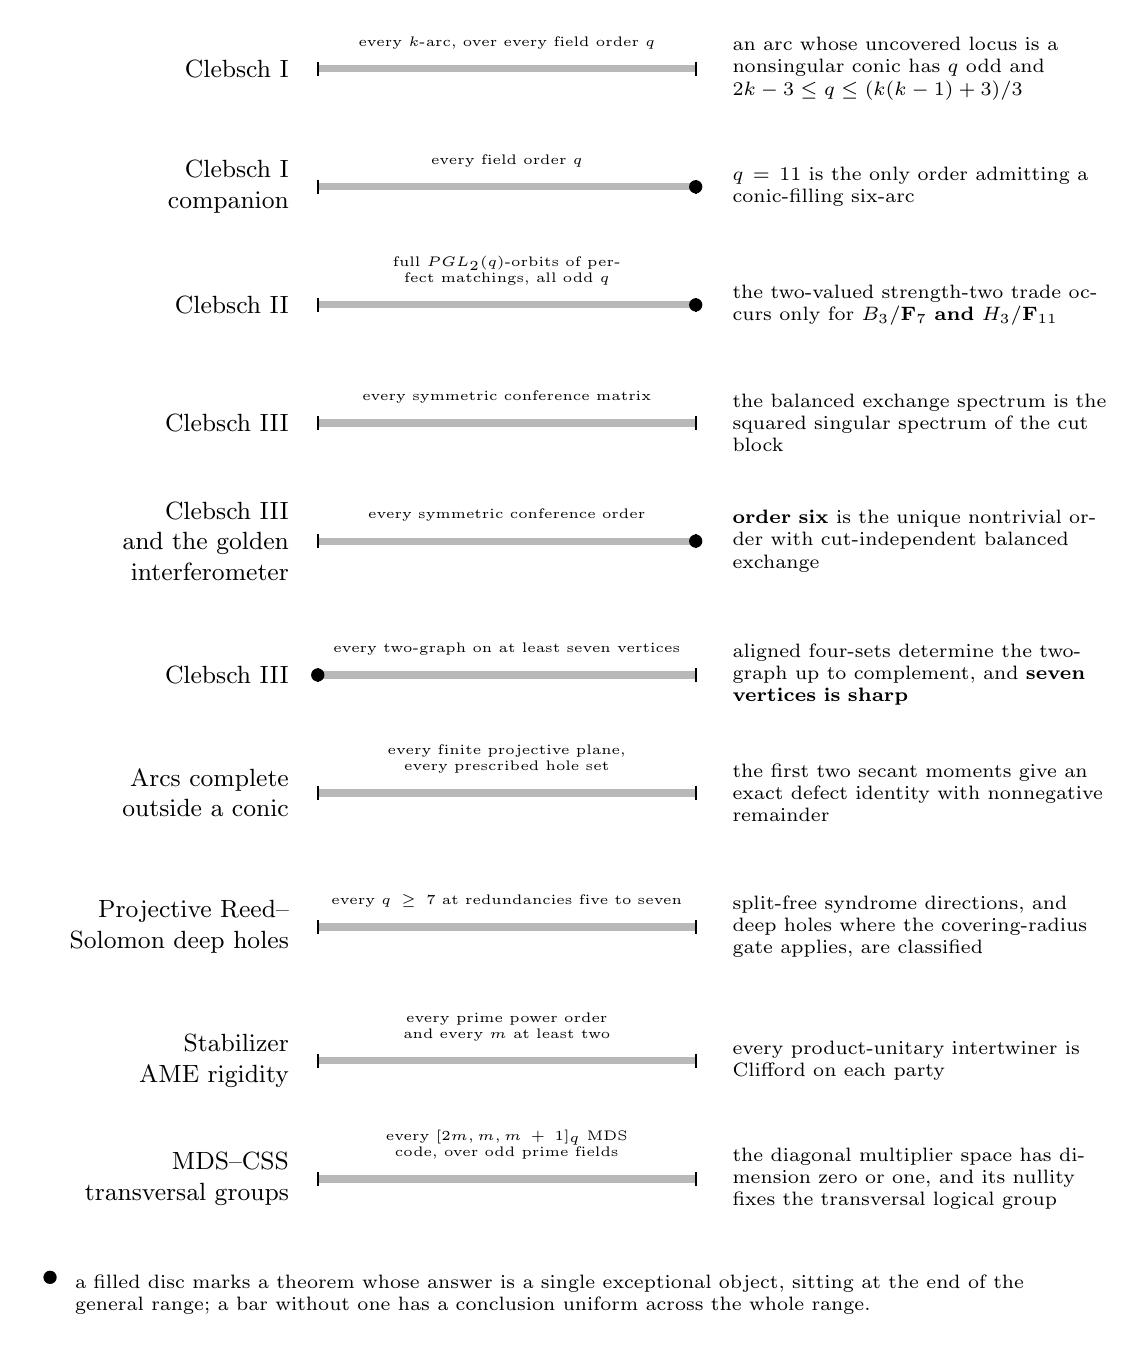
\begin{tikzpicture}[every node/.style={outer sep=0pt}]

\ClebschLadderRow{0}{Clebsch I}
  {every \(k\)-arc, over every field order \(q\)}
  {an arc whose uncovered locus is a nonsingular conic has \(q\) odd and
   \(2k-3\le q\le (k(k-1)+3)/3\)}{n}

\ClebschLadderRow{-1.5}{Clebsch I\\companion}
  {every field order \(q\)}
  {\textbf{\(q=11\)} is the only order admitting a conic-filling six-arc}{r}

\ClebschLadderRow{-3.0}{Clebsch II}
  {full \(\operatorname{PGL}_2(q)\)-orbits of perfect matchings, all odd \(q\)}
  {the two-valued strength-two trade occurs only for
   \textbf{\(B_3/\mathbf F_7\) and \(H_3/\mathbf F_{11}\)}}{r}

\ClebschLadderRow{-4.5}{Clebsch III}
  {every symmetric conference matrix}
  {the balanced exchange spectrum is the squared singular spectrum of the
   cut block}{n}

\ClebschLadderRow{-6.0}{Clebsch III\\and the golden interferometer}
  {every symmetric conference order}
  {\textbf{order six} is the unique nontrivial order with cut-independent
   balanced exchange}{r}

\ClebschLadderRow{-7.7}{Clebsch III}
  {every two-graph on at least seven vertices}
  {aligned four-sets determine the two-graph up to complement, and
   \textbf{seven vertices is sharp}}{l}

\ClebschLadderRow{-9.2}{Arcs complete outside a conic}
  {every finite projective plane, every prescribed hole set}
  {the first two secant moments give an exact defect identity with
   nonnegative remainder}{n}

\ClebschLadderRow{-10.9}{Projective Reed--Solomon deep holes}
  {every \(q\ge7\) at redundancies five to seven}
  {split-free syndrome directions, and deep holes where the
   covering-radius gate applies, are classified}{n}

\ClebschLadderRow{-12.6}{Stabilizer AME rigidity}
  {every prime power order and every \(m\) at least two}
  {every product-unitary intertwiner is Clifford on each party}{n}

\ClebschLadderRow{-14.1}{MDS--CSS transversal groups}
  {every \([2m,m,m+1]_q\) MDS code, over odd prime fields}
  {the diagonal multiplier space has dimension zero or one, and its
   nullity fixes the transversal logical group}{n}

\fill (-7.3,-15.35) circle (2.4pt);
\node[anchor=north west,font=\scriptsize,align=left,text width=124mm]
  at (-7.1,-15.2)
  {a filled disc marks a theorem whose answer is a single exceptional
   object, sitting at the end of the general range; a bar without one has a
   conclusion uniform across the whole range.};

\end{tikzpicture}%
}
